\documentclass[11pt, a4paper]{article}
\usepackage{pdfpages}
\usepackage{parallel}
\usepackage[T2A]{fontenc}
\usepackage{ucs}
\usepackage[utf8x]{inputenc}
\usepackage[polish,english,russian]{babel}
\usepackage{hyperref}
\usepackage{rotating}
\usepackage[inner=2cm,top=1.8cm,outer=2cm,bottom=2.3cm,nohead]{geometry}
\usepackage{listings}
\usepackage{graphicx}
\usepackage{wrapfig}
\usepackage{longtable}
\usepackage{indentfirst}
\usepackage{array}
\usepackage{tikzsymbols}
\usepackage{soul}
\usepackage[ruled,vlined]{algorithm2e}
%\counterwithout{figure}{section} 

\usepackage{url}
\makeatletter
\g@addto@macro{\UrlBreaks}{\UrlOrds}
\makeatother

\newcolumntype{P}[1]{>{\raggedright\arraybackslash}p{#1}}
\frenchspacing
\usepackage{fixltx2e} %text sub- and superscripts
\usepackage{icomma} % коскі ў матэматычным рэжыме
\PreloadUnicodePage{4}

\newcommand{\longpage}{\enlargethispage{\baselineskip}}
\newcommand{\shortpage}{\enlargethispage{-\baselineskip}}

\def\switchlang#1{\expandafter\csname switchlang#1\endcsname}
\def\switchlangbe{
\let\saverefname=\refname%
\def\refname{Літаратура}%
\def\figurename{Іл.}%
}
\def\switchlangen{
\let\saverefname=\refname%
\def\refname{References}%
\def\figurename{Fig.}%
}
\def\switchlangru{
\let\saverefname=\refname%
\let\savefigurename=\figurename%
\def\refname{Литература}%
\def\figurename{Рис.}%
}

\hyphenation{admi-ni-stra-tive}
\hyphenation{ex-pe-ri-ence}
\hyphenation{fle-xi-bi-li-ty}
\hyphenation{Py-thon}
\hyphenation{ma-the-ma-ti-cal}
\hyphenation{re-ported}
\hyphenation{imp-le-menta-tions}
\hyphenation{pro-vides}
\hyphenation{en-gi-neering}
\hyphenation{com-pa-ti-bi-li-ty}
\hyphenation{im-pos-sible}
\hyphenation{desk-top}
\hyphenation{elec-tro-nic}
\hyphenation{com-pa-ny}
\hyphenation{de-ve-lop-ment}
\hyphenation{de-ve-loping}
\hyphenation{de-ve-lop}
\hyphenation{da-ta-ba-se}
\hyphenation{plat-forms}
\hyphenation{or-ga-ni-za-tion}
\hyphenation{pro-gramming}
\hyphenation{in-stru-ments}
\hyphenation{Li-nux}
\hyphenation{sour-ce}
\hyphenation{en-vi-ron-ment}
\hyphenation{Te-le-pathy}
\hyphenation{Li-nux-ov-ka}
\hyphenation{Open-BSD}
\hyphenation{Free-BSD}
\hyphenation{men-ti-on-ed}
\hyphenation{app-li-ca-tion}

\def\progref!#1!{\texttt{#1}}
\renewcommand{\arraystretch}{2} %Іначай формулы ў матрыцы зліпаюцца з лініямі
\usepackage{array}

\def\interview #1 (#2), #3, #4, #5\par{

\section[#1, #3, #4]{#1 -- #3, #4}
\def\qname{LVEE}
\def\aname{#1}
\def\q ##1\par{{\noindent \bf \qname: ##1 }\par}
\def\a{{\noindent \bf \aname: } \def\qname{L}\def\aname{#2}}
}

\def\interview* #1 (#2), #3, #4, #5\par{

\section*{#1\\{\small\rm #3, #4. #5}}
\ifx\ParallelWhichBox\undefined%
    \addcontentsline{toc}{section}{#1, #3, #4}%
\else%
\ifnum\ParallelWhichBox=0%
    \addcontentsline{toc}{section}{#1, #3, #4}%
\fi\fi%

\def\qname{LVEE}
\def\aname{#1}
\def\q ##1\par{{\noindent \bf \qname: ##1 }\par}
\def\a{{\noindent \bf \aname: } \def\qname{L}\def\aname{#2}}
}

\newcommand{\interviewfooter}[1]{
\vskip 1em
\noindent \textit{#1}
}

\switchlang{ru}
\begin{document}

\title{1988 "--- Mouse Systems M4 PC mouse}
\date{}
\maketitle
\selectlanguage{russian}
Mouse Systems M4 mouse (рис. \ref{fig:mscM4Pic}) "--- характерный манипулятор компании Mouse Systems, созданной Стивеном Киршем в 1982 году для производства изобретенной им оригинальной оптической мыши. Данная версия "--- представитель четвертого (последнего и самого массового) поколения мышей Mouse Systems конструкции Кирша, адаптированный для работы с последовательным интерфейсом IBM PC, RS-232.

\begin{figure}[h]
    \centering
    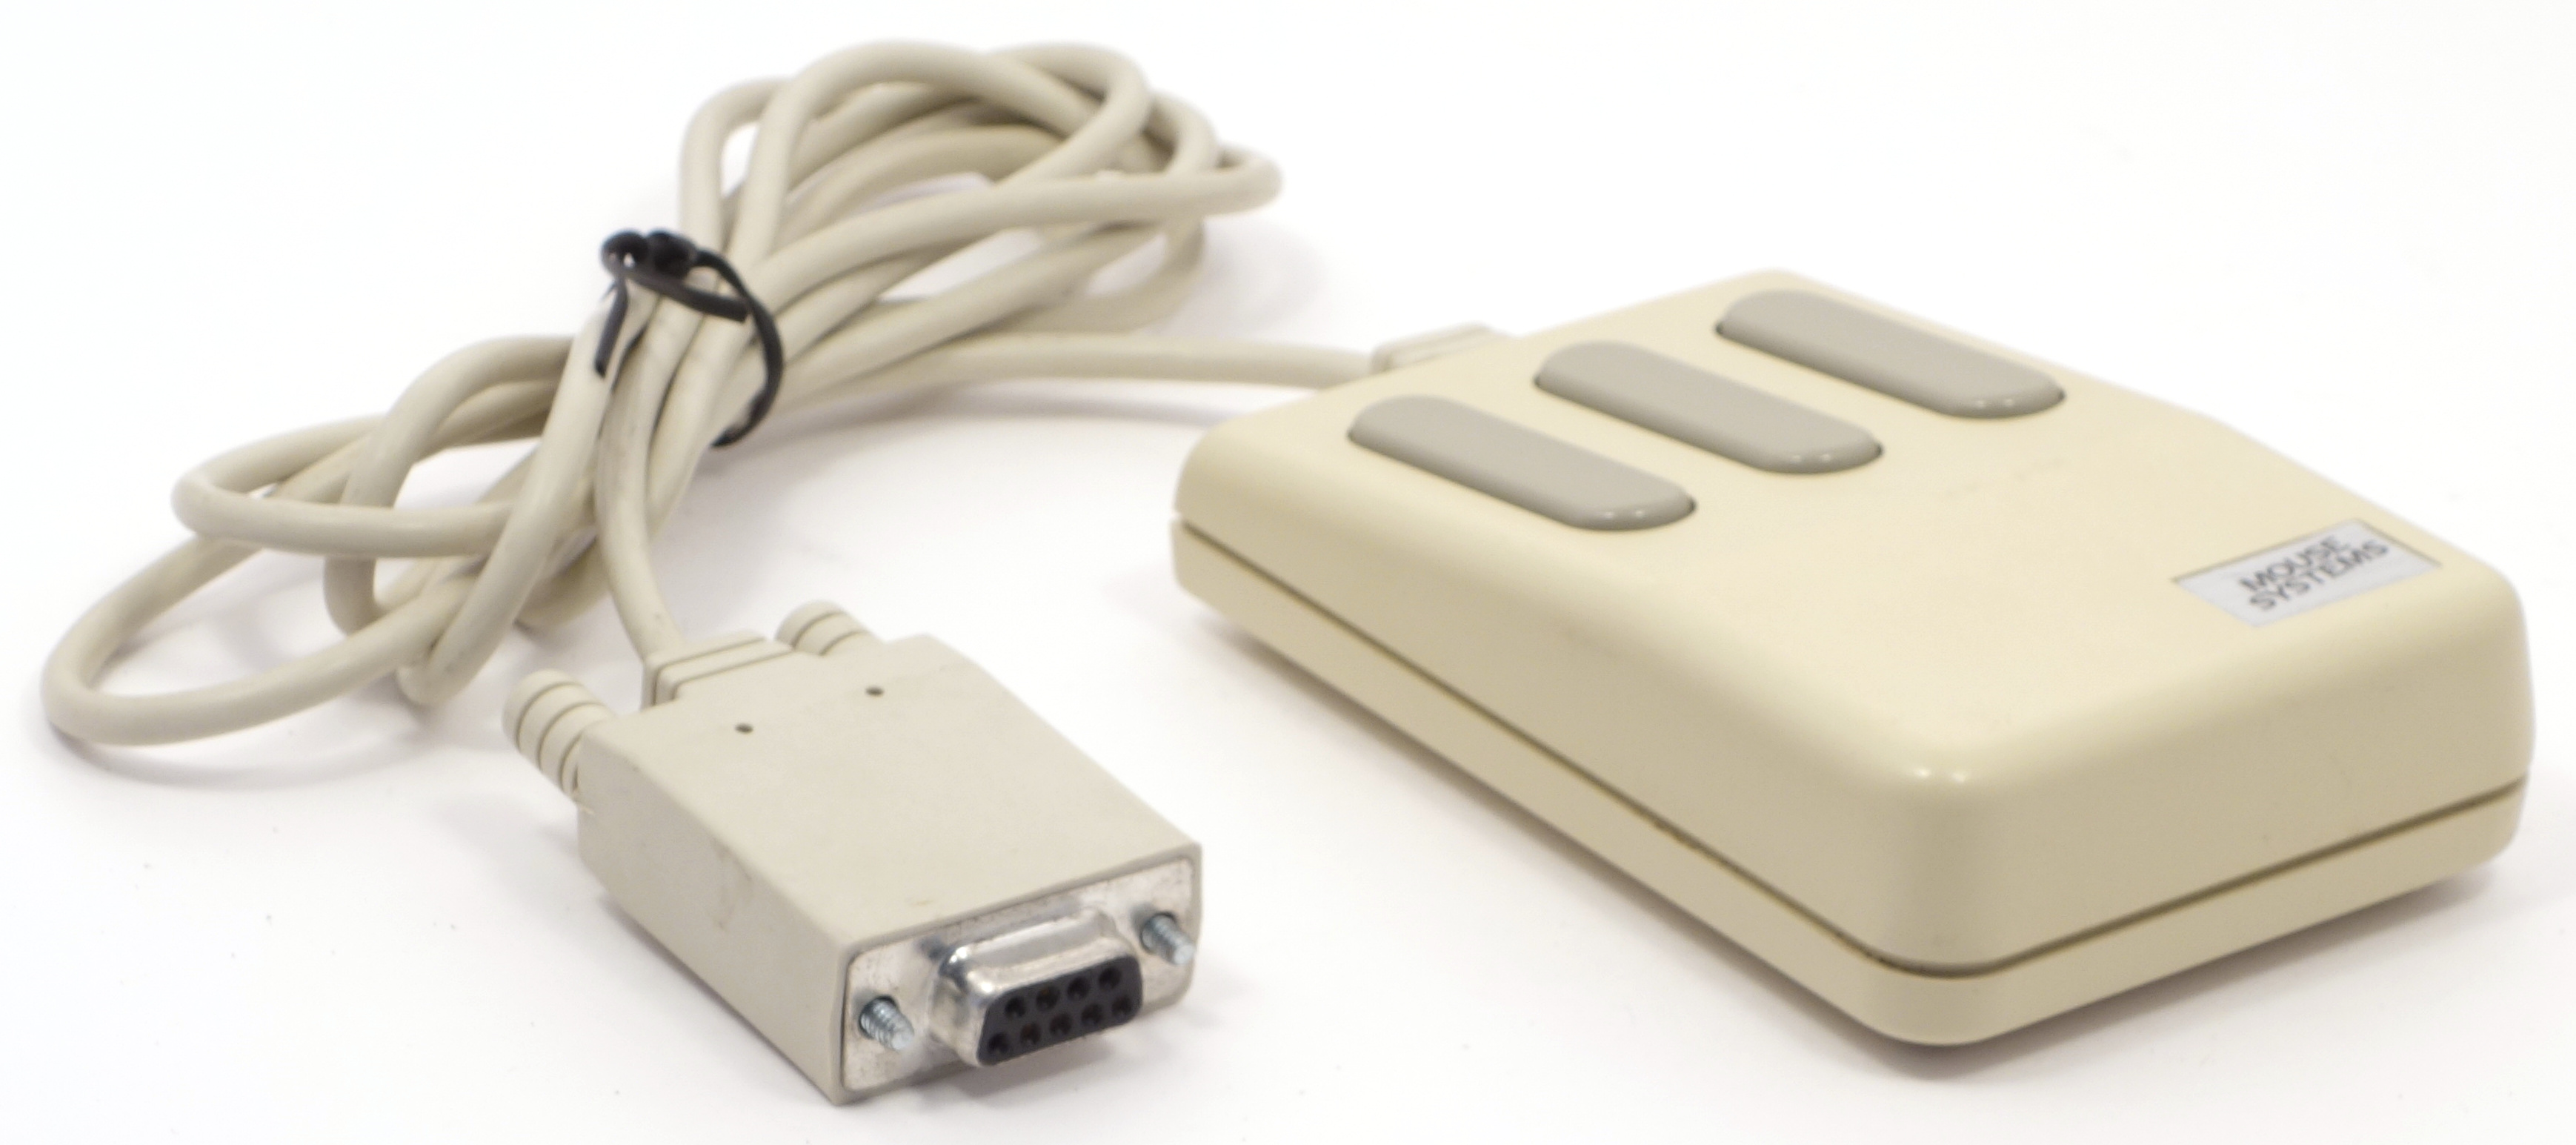
\includegraphics[scale=0.5]{1988_mouse_systems_m4/pic_30.jpg}
    \caption{Мышь Mouse Systems M4}
    \label{fig:mscM4Pic}
\end{figure}

Как всем ранним оптическим мышам, данному манипулятору требуется коврик с отражающей сеткой (рис. \ref{fig:mscM4Pad}). Это традиционный металлический коврик Mouse Systems с решеткой из вертикальных и горизонтальных линий, соответствующих двум разным длинам волн (в оптическом и в инфракрасном диапазоне).

\begin{figure}[h]
    \centering
    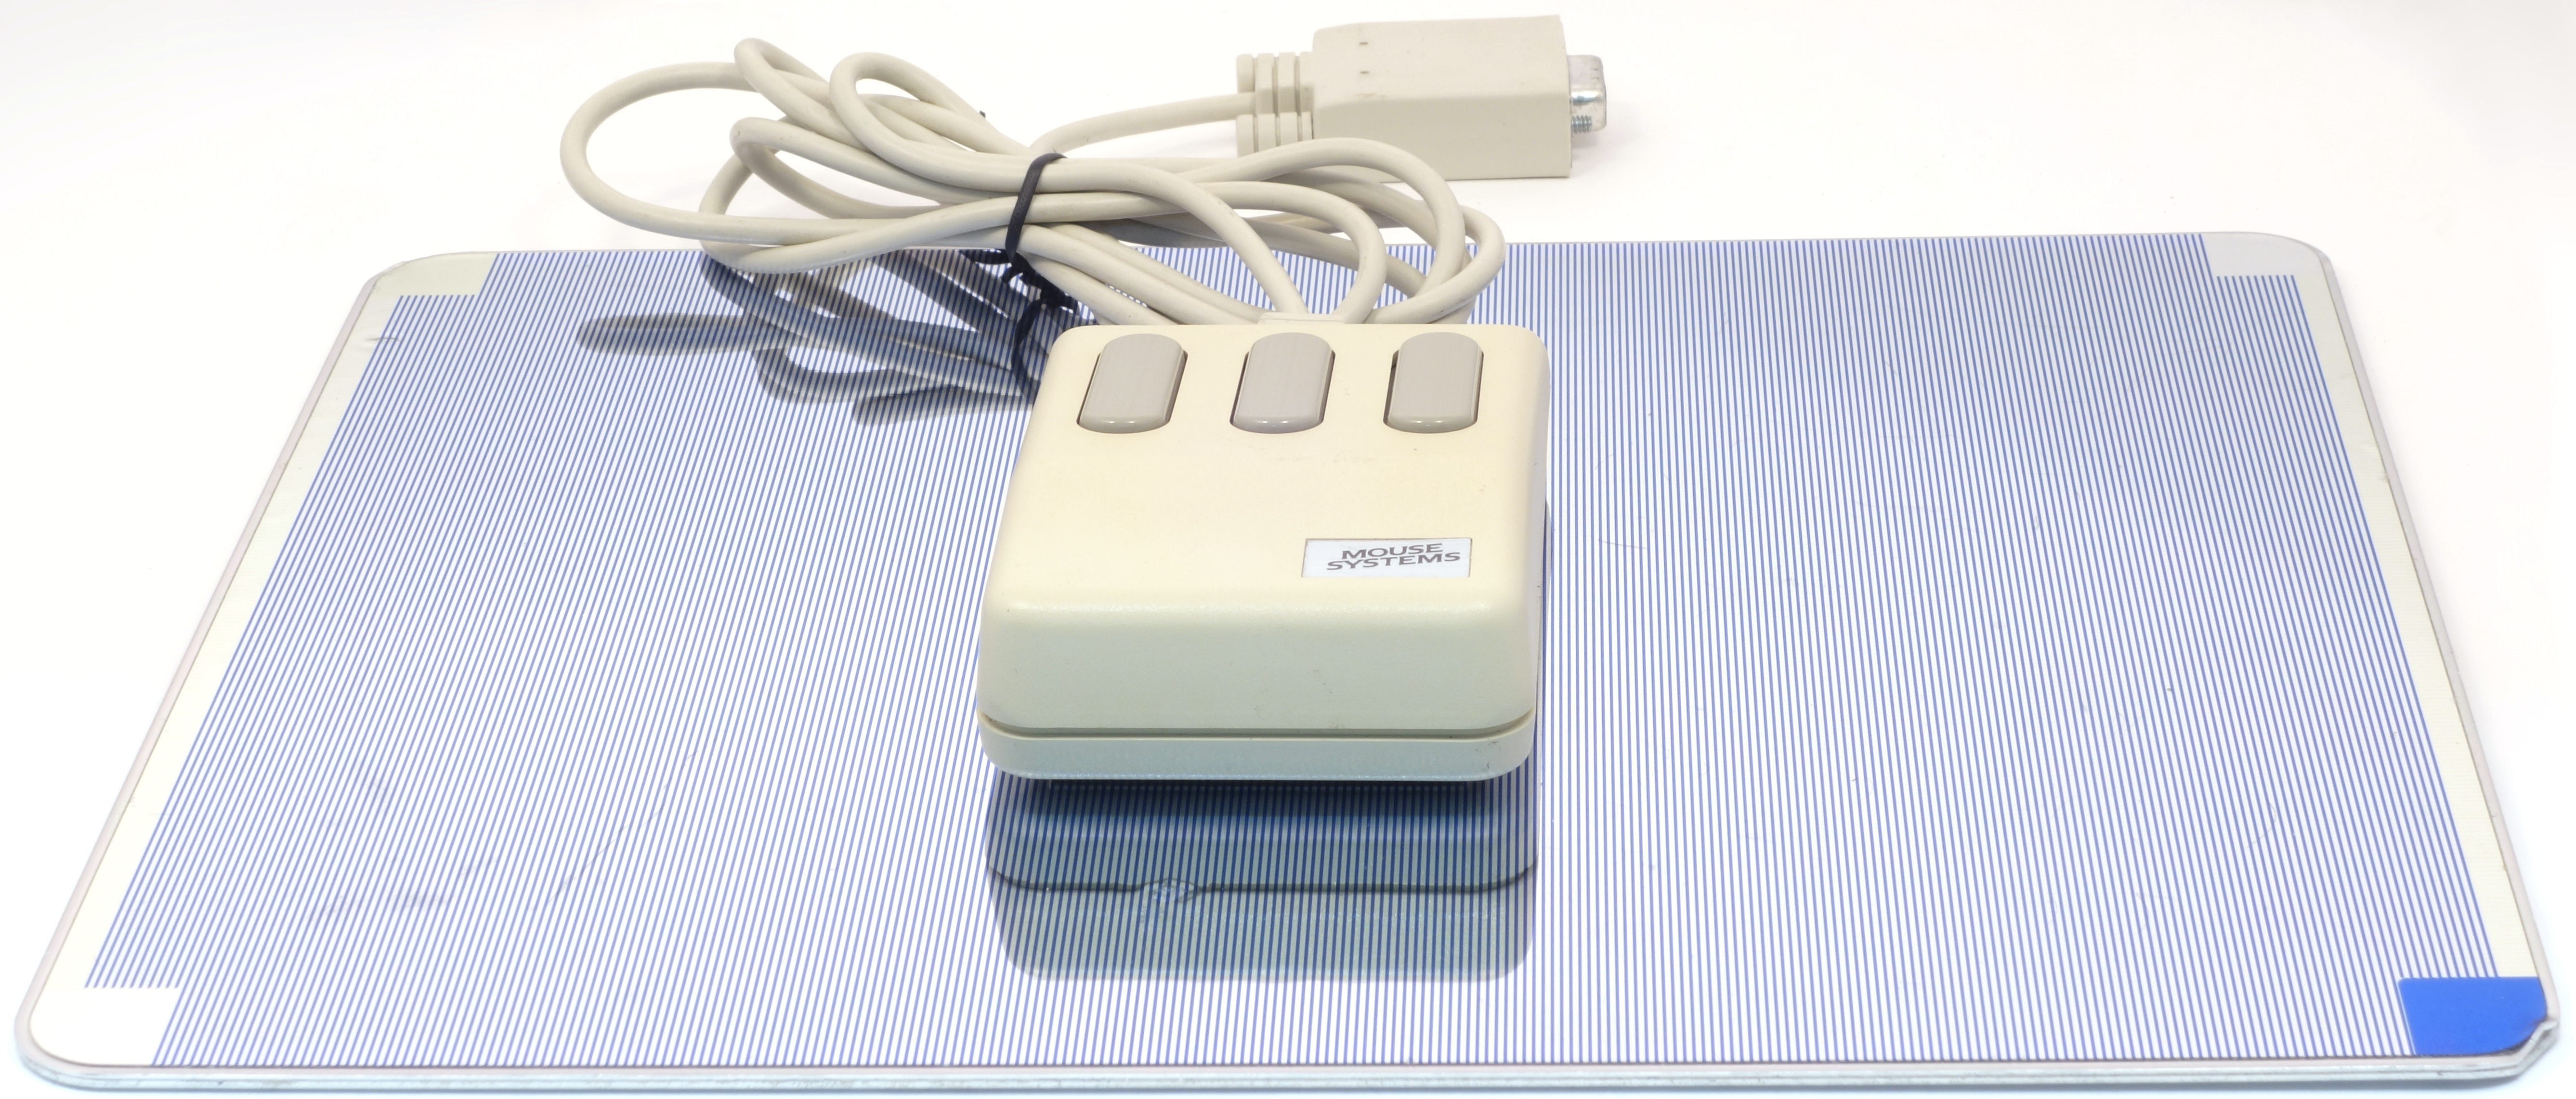
\includegraphics[scale=0.4]{1988_mouse_systems_m4/pad_30.jpg}
    \caption{Мышь Mouse Systems M4 на комплектном коврике}
    \label{fig:mscM4Pad}
\end{figure}

Мышь выполнена в стандартном для Mouse Systems плоском прямоугольном корпусе с тремя вытянутыми закругленными кнопками. На верхней стороне корпуса присутствует табличка с названием компании MOUSE SYSTEMS, набранным курсивом, на нижней стороне "--- то же название и эмблема в виде двух треугольников, стилизованных под изображение мыши и экранного курсора (рис. \ref{fig:mscM4TopBottom}). В отличие от ранних моделей мышей Mouse Systems с интерфейсом RS-232 (например, мыши M2) Мышь M4 использует менее энергоемкие светодиоды и потому не требует дополнительного блока питания.

Изучение кода FCC ID по базе данных Федеральной комиссии по связи США показывает, что мышь была выпущена компанией Mouse Systems в 1988 году.

\begin{figure}[h]
    \centering
    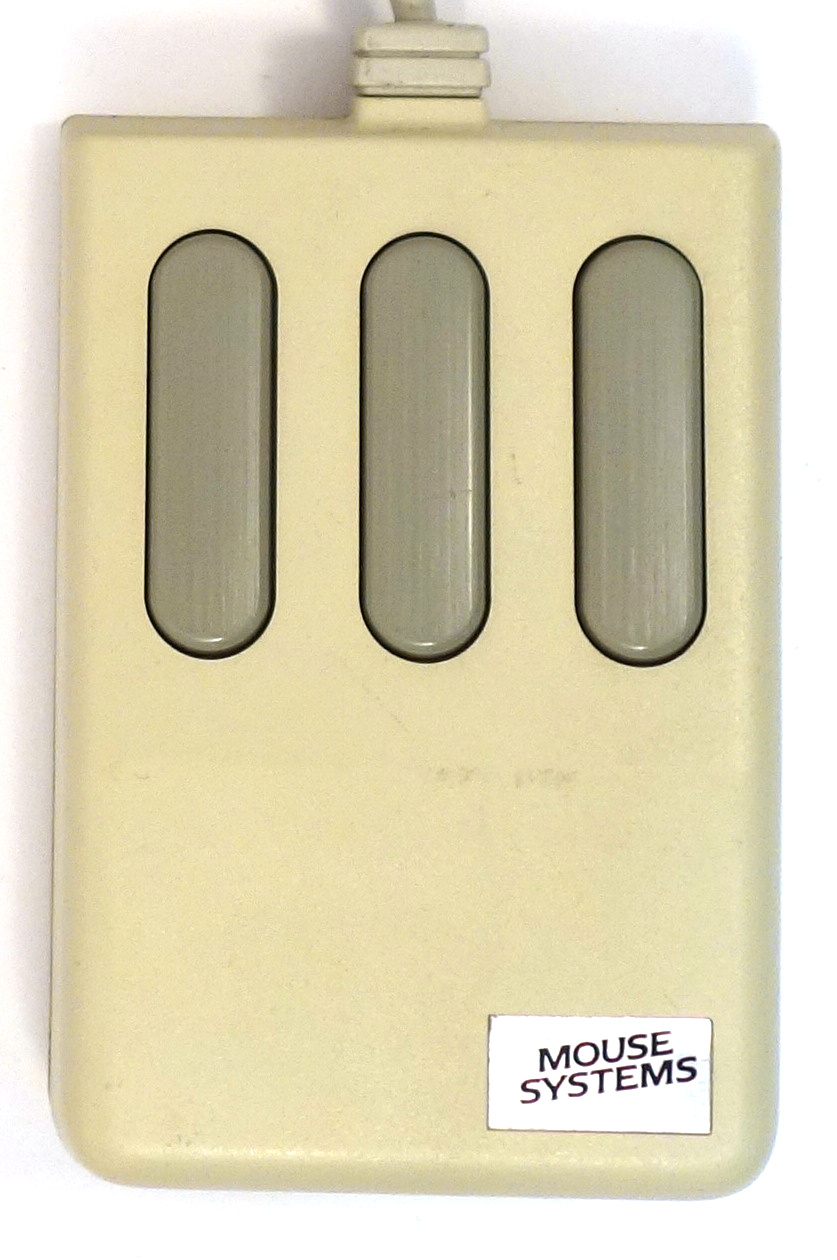
\includegraphics[scale=0.6]{1988_mouse_systems_m4/top_30.jpg}
    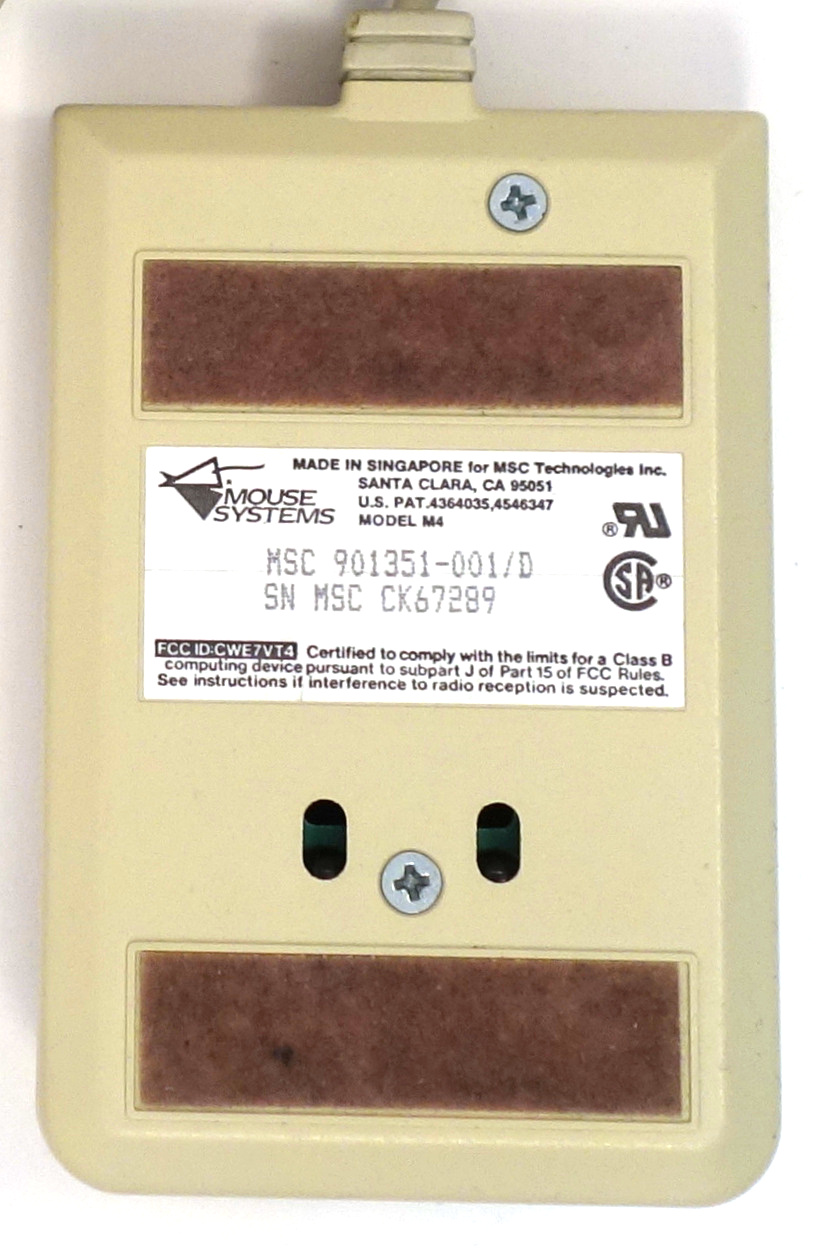
\includegraphics[scale=0.6]{1988_mouse_systems_m4/bottom_30.jpg}
    \caption{Мышь Mouse Systems M4, вид сверху и снизу}
    \label{fig:mscM4TopBottom}
\end{figure}

Некрупный, подчеркнуто плоский корпус (рис. \ref{fig:mscM4Size}) наглядно иллюстрирует отсутствие шара и других механических элементов \cite{pcmag}; он оказался достаточно удачен и не претерпел изменений в размерах и форме начиная с первого поколения мышей компании \cite{old}.

\begin{figure}[h]
    \centering
    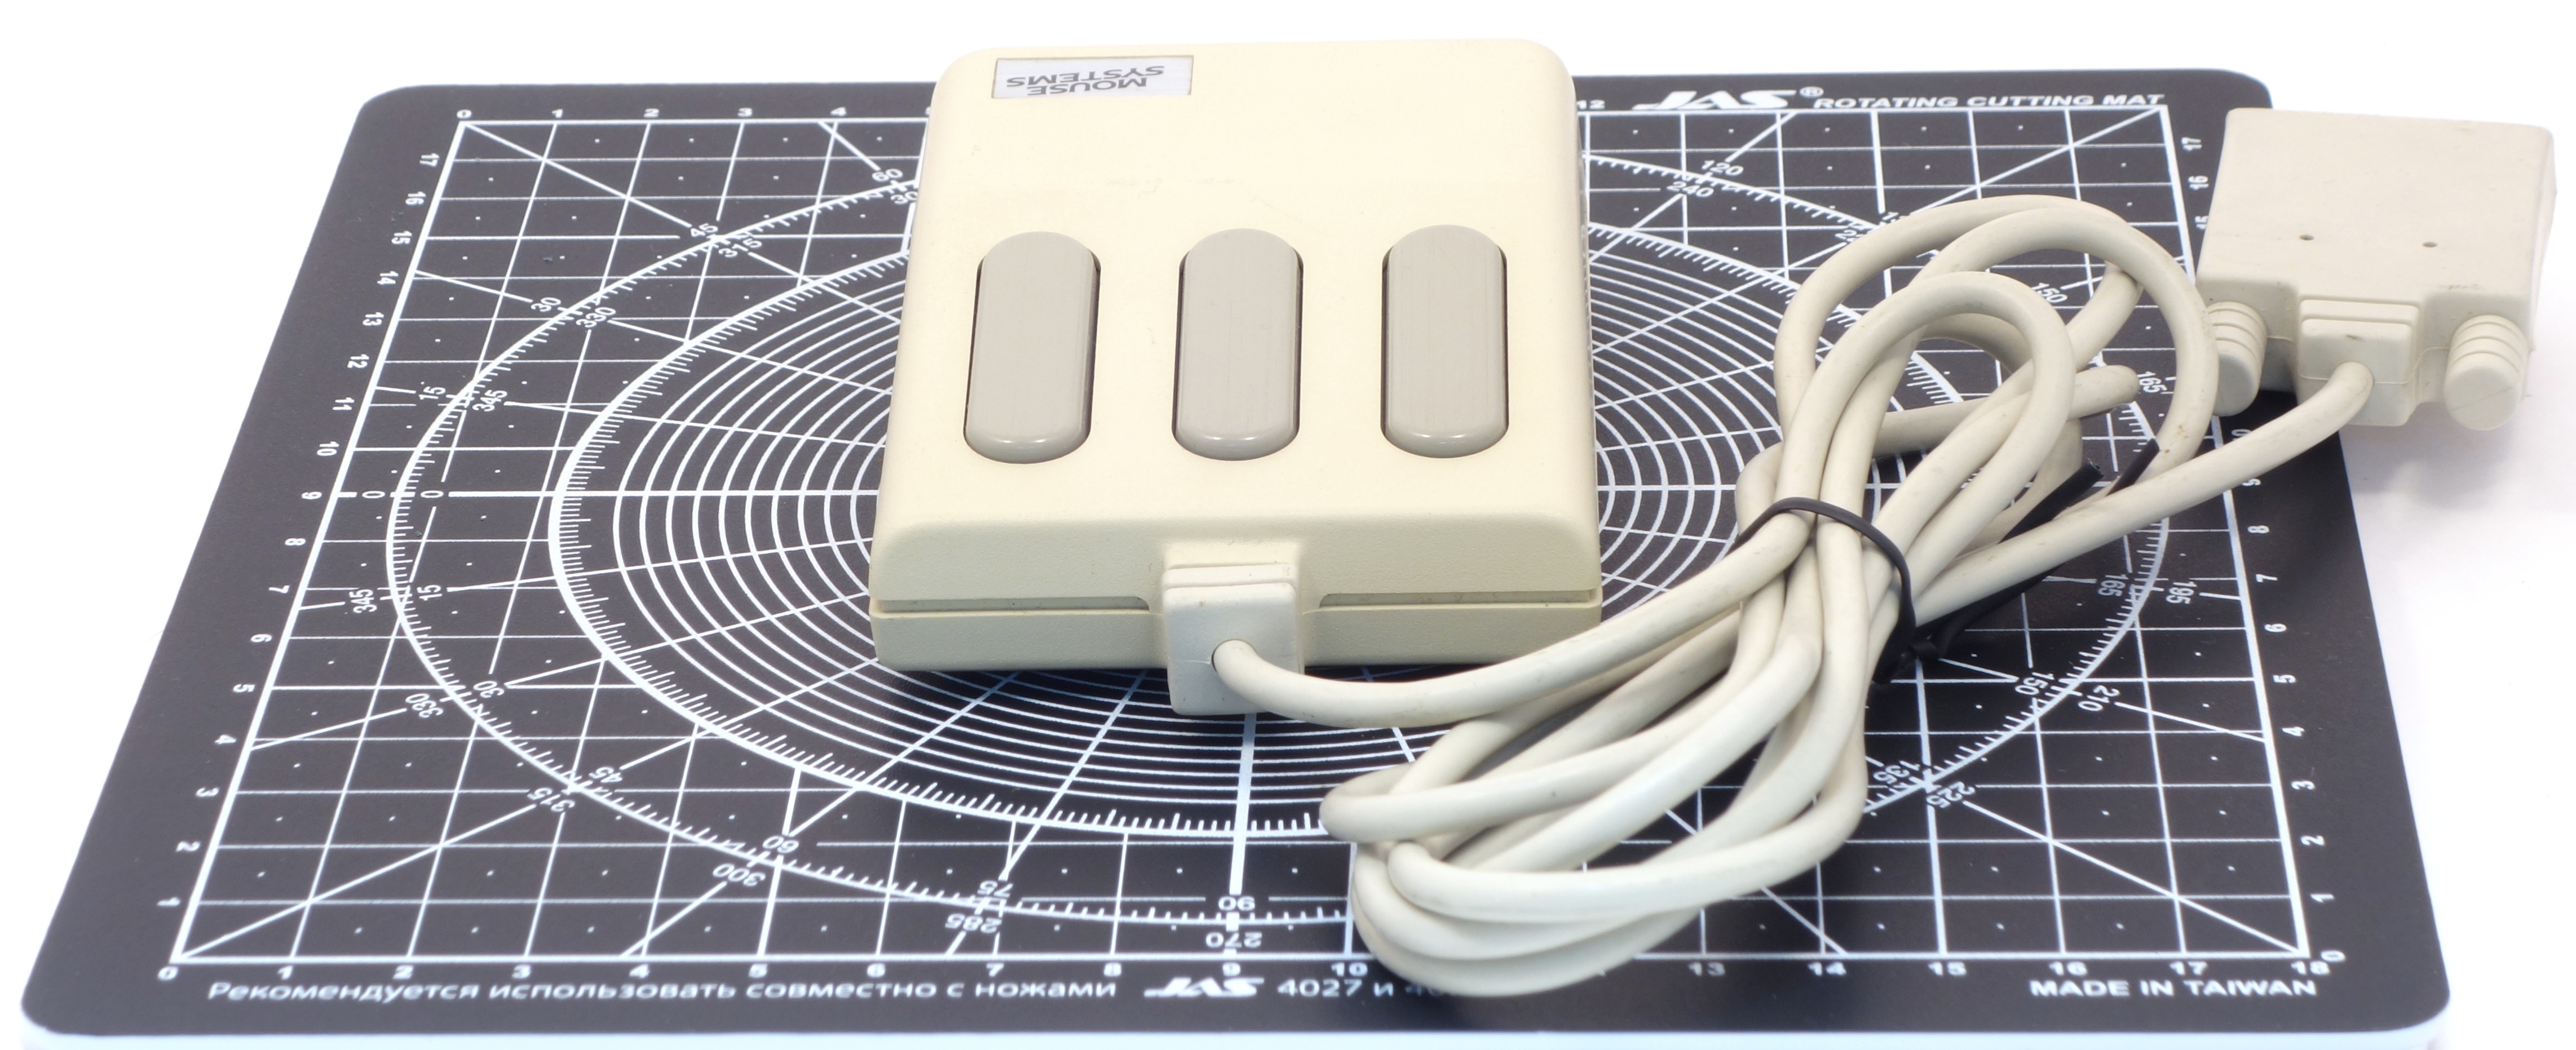
\includegraphics[scale=0.5]{1988_mouse_systems_m4/size_30.jpg}
    \caption{Mouse Systems M4 на размерном коврике с шагом сетки 1~см}
    \label{fig:mscM4Size}
\end{figure}

Мышь имеет достаточно эргономичную по меркам 80-х годов форму (рис. \ref{fig:mscM4Hand}) благодаря достаточно удачной форме с закругленными углами и большими кнопками. Отсутствие опоры под запястье отчасти компенсируется малой высотой корпуса мыши, а кнопки входят в число самых эргономичных среди манипуляторов восьмидесятых.

\begin{figure}[h]
    \centering
    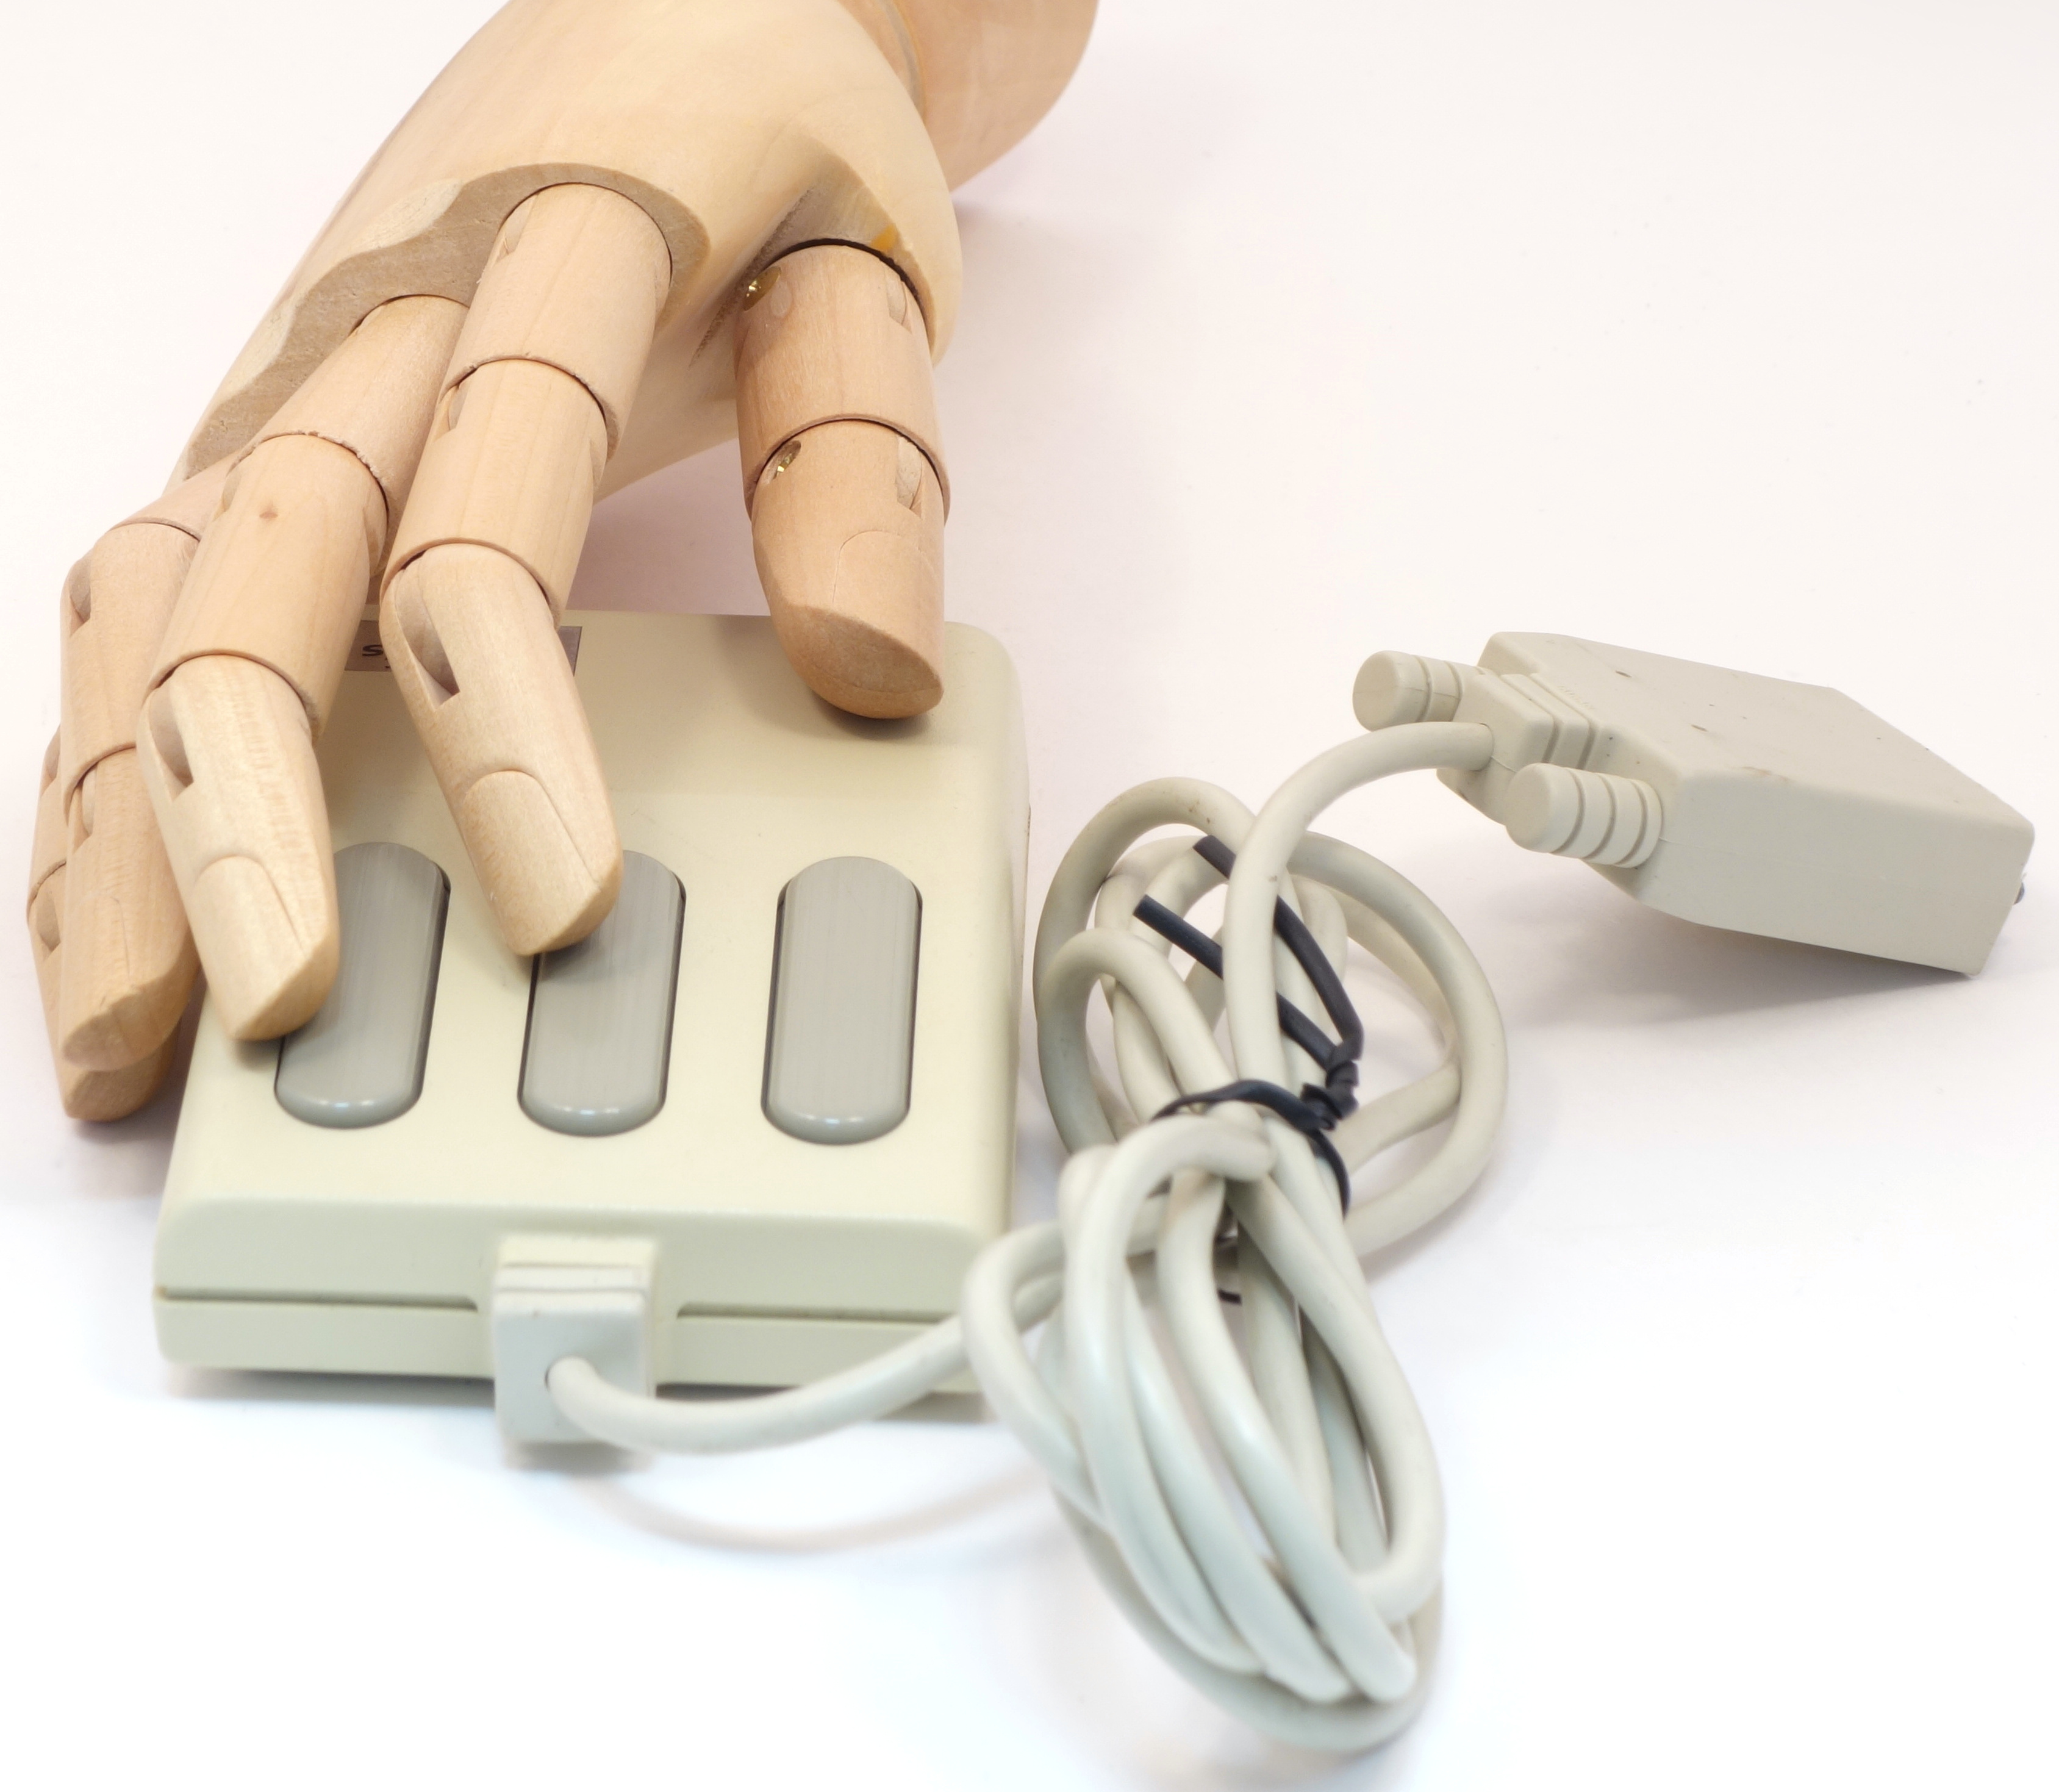
\includegraphics[scale=0.35]{1988_mouse_systems_m4/hand_30.jpg}
    \caption{Mouse Systems M4 с моделью руки человека}
    \label{fig:mscM4Hand}
\end{figure}

Внутреннее устройство показано на рис. \ref{fig:mscM4Inside}.
В соответствии с придуманной Киршем схемой, излучаемый светодиодами свет отражается от коврика, затем от блестящей фольгированной пластины в верхней части корпуса мыши, и наконец попадает на две линейки фотоприемников, одна из которых расположена вдоль продольной оси, а другая "--- вдоль поперечной. Один из светодиодов излучает свет в оптическом диапазоне, в котором видны нанесенные на коврик поперечные линии, а другой "--- в инфракрасном, в котором считываются не поперечные, а продольные линии. В результате движения чередование линий считывается соответствующей линейкой фотоприемников. На рис. \ref{fig:mscM4Inside} можно увидеть две линейки фотоприемников (по 4 в каждой): это  усовершенствованная по сравнению с исходным вариантом Стивена Кирша конструкция (в первом поколении мышей Mouse Systems использовалась единственная матрица фотоприемников размером $2 \times 2$, недостатком которой был период калибровки мыши после каждого включения, во время которого микроконтроллер выполнял автоподбор корректных пороговых значений срабатывания фотодатчиков) \cite{bio}.

\begin{figure}[h]
    \centering
    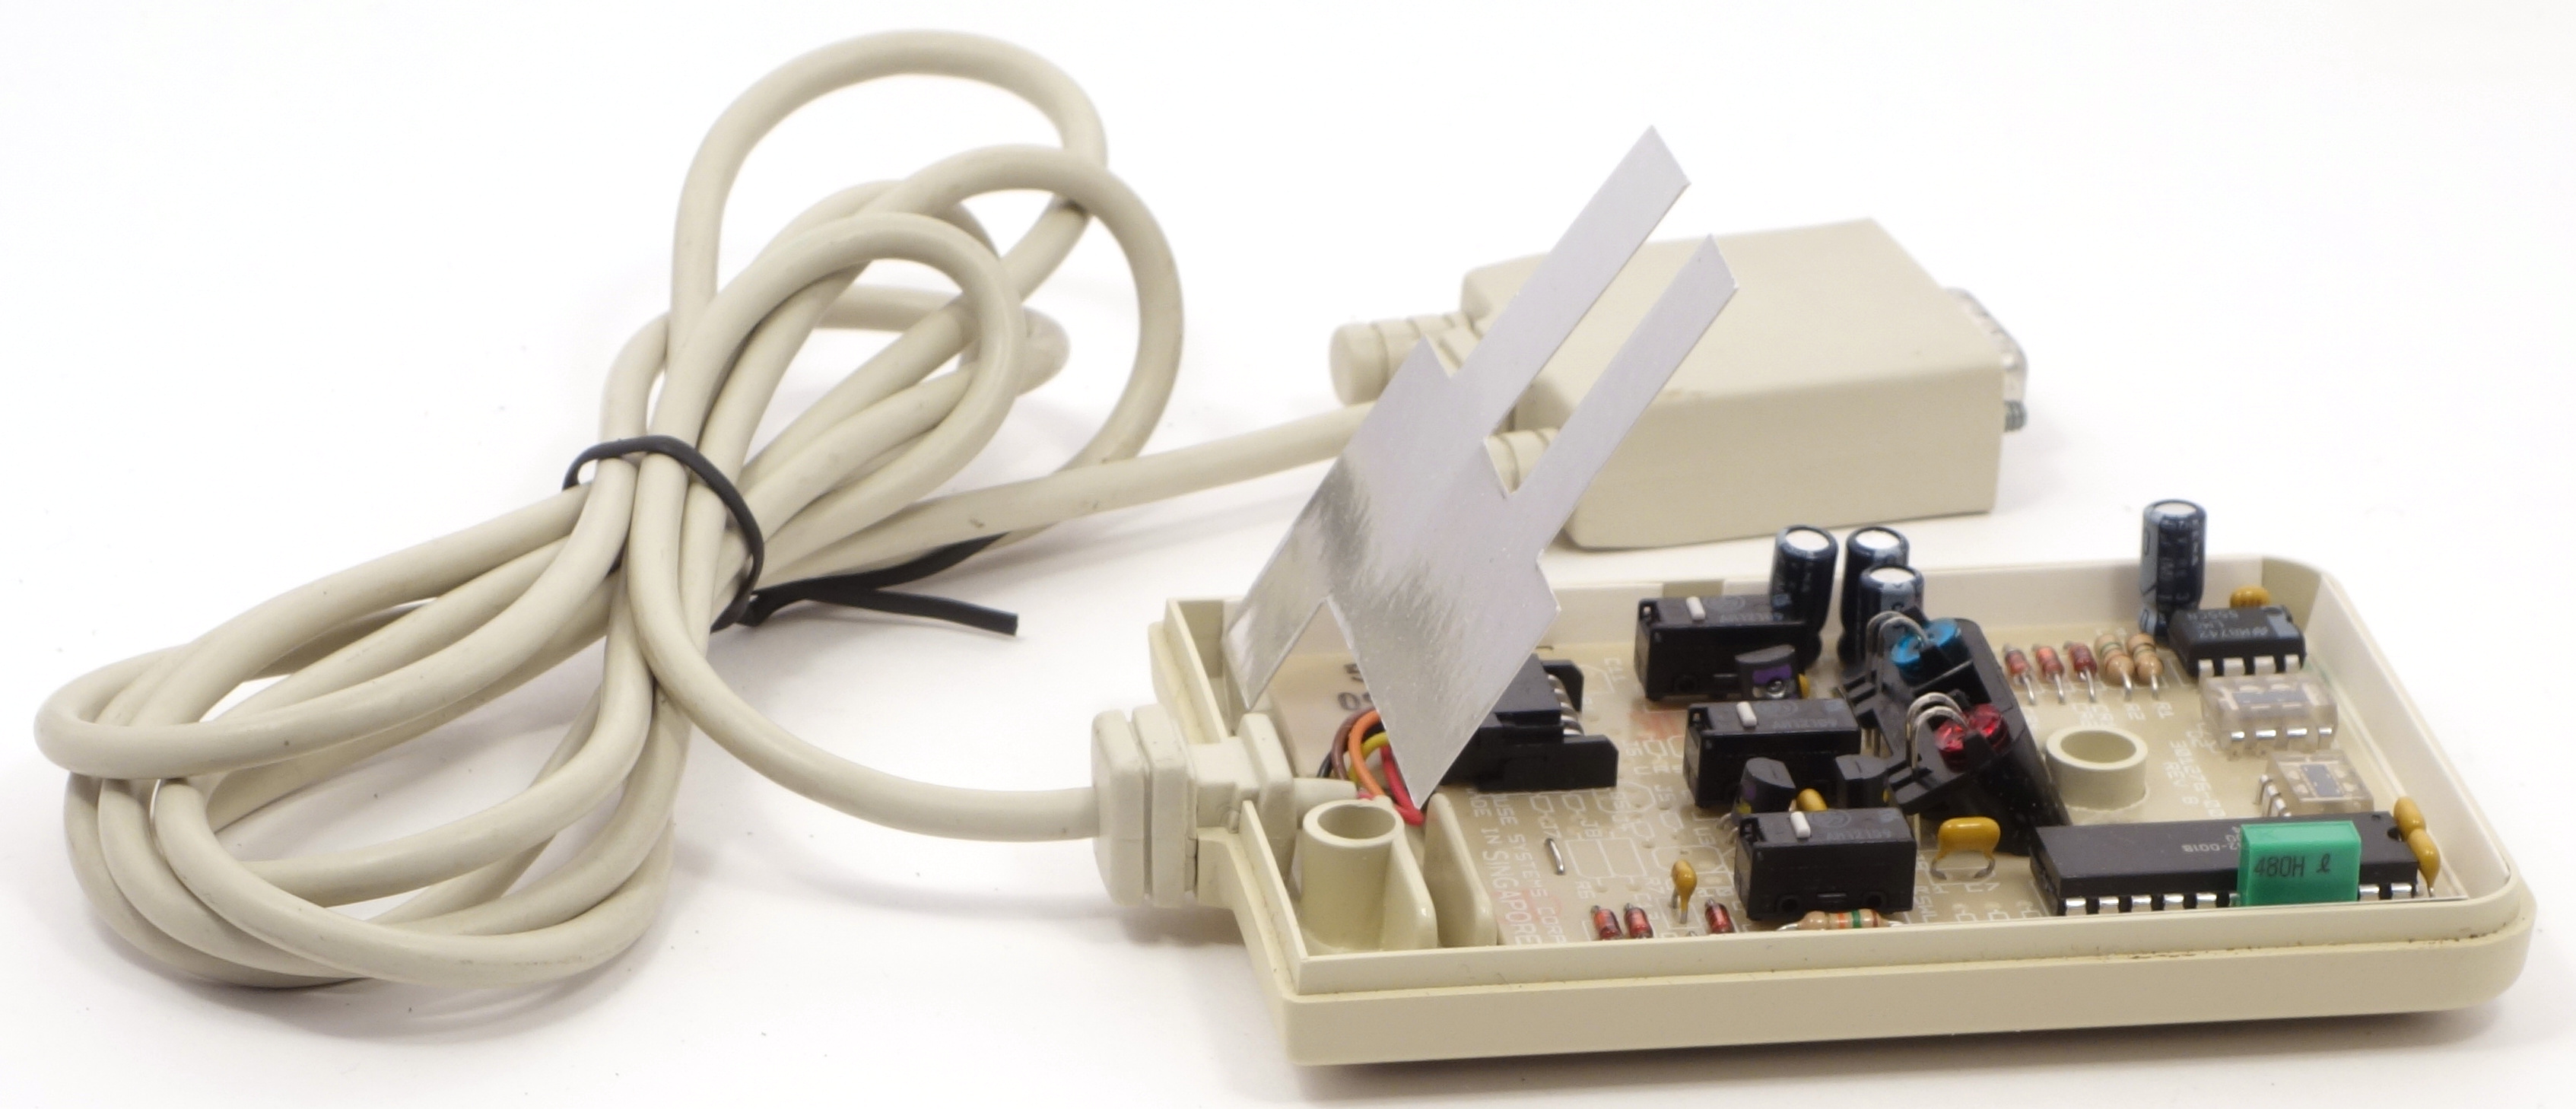
\includegraphics[scale=0.6]{1988_mouse_systems_m4/inside_30.jpg}
    \caption{Mouse Systems M4 mouse в разобранном виде}
    \label{fig:mscM4Inside}
\end{figure}


\begin{thebibliography}{9}
\bibitem {pcmag} Why you should buy the mouse with no moving parts [adv.] // PC MAGAZINE, V. 7, No. 3, February 16, 1988. P. 205. \url{https://archive.org/details/PC-Mag-1988-02-16/page/n203/mode/2up}
\bibitem {old} Mouse Systems -- oldmouse.com  \url{https://web.archive.org/web/20211205082304/http://oldmouse.com/mouse/mousesystems/}
\bibitem {bio} Perry S.T. Steve Kirsch -- IEEE Spectrum. 01 AUG 2000 \url{https://spectrum.ieee.org/steve-kirsch}
\end{thebibliography}
\end{document}
